\documentclass[a4paper,11pt]{article}

\usepackage[top=2.5cm , bottom=3cm, left = 2.5cm, right = 2.5cm]{geometry}
\usepackage{tikz}
\usepackage{graphicx}
\usepackage{amsmath}
\usepackage{caption, subfig}
 \usepackage{booktabs}
 \usepackage{multirow, makecell}  %add some packages
\usetikzlibrary{shapes,arrows.meta,positioning}

\linespread{1.25}
\usepackage{enumerate, titling}
\usepackage{color,xcolor}
\usepackage[flushleft]{threeparttable}
\usepackage{amsmath, graphicx, hyperref, lipsum}
\hypersetup{
    colorlinks=true,
    linkcolor=blue,
    filecolor=magenta,      
    urlcolor=cyan}
\usepackage[authordate,natbib]{biblatex-chicago}
\addbibresource{moonopoly.bib}


\title{\vspace{-1.2cm} Market Concentration and Competition in the Canadian Dental Industry} 
\author{Emily Hanson, Zhaoqi Li, Shuning Li, Nalinda Murray, Lance Taylor }
\date{May 10, 2024}

\begin{document}


\maketitle \vspace{-.4 in}
\begin{center}
University of Western Ontario
\rule{\textwidth}{1pt} 
\end{center}




\begin{abstract}
\textit{``We did more or less what we were asked to do."} - Lance Taylor.
\end{abstract}

\section{Introduction}
The 2022 Canadian Community Health Survey revealed that over one-third of Canadians did not receive dental care services in the year preceding the survey, despite a recommended frequency of two dental exams per year in order to maintain good oral health \citep{StatisticsCanada}. The survey also revealed a sizeable gap in visits to dental professionals by income: 73\% of surveyed Canadians in the highest income quintile reported having visited a dental professional in the past year, compared to only 45\% of Canadians in the lowest income quintile. Infrequent dental visits among Canadians, especially by income, may be explained in part by difficulty affording dental care. The survey suggests that approximately one in four Canadians avoid seeing dental professionals due to the cost, and this is typically worse for marginalized and immigrant groups. Additionally, more than one in three Canadians do not have any private nor public dental insurance coverage and would have to pay for services out-of-pocket.

Notably, dental services are relatively costly in Canada. Among G7 countries, Canada (414 USD) ranks second to the U.S. (518 USD) in average prices of dental services \citep{Sankovich} and is followed by the U.K. (331 USD).\footnote{These country price averages were computed across five key dental treatments: cleanings, crowns, root canals, tooth extractions, and fillings.} The level of dental care expenses is clearly an important issue for Canadians, especially in recent years, as the federal government launched the Canada Dental Benefit in December 2022 to provide coverage for children under twelve years of age whose parents do not have private insurance. This program, now called the Canadian Dental Care Plan (CDCP), has since been expanded to provide coverage to uninsured Canadians under eighteen years of age, those with disabilities, and senior citizens satisfying a specific income criteria. The final expansion to working-age Canadians satisfying a specific income criteria is expected to take place by 2025. Providing insurance coverage for a quarter of Canadians, the plan is expected to cost approximately 4.4 billion CAD per year \citep{Rachini}.

Despite the recent roll-out of the CDCP to senior Canadians, participation of dentists in the program is currently low, which may be due to the fact that the program requires participating dental clinics to provide services at lower rates for those covered by the CDCP \citep{vonStackelberg}. The apparent reluctance of dentists to participate in the CDCP may be particularly worrisome for Canadians living in more isolated towns, who may lack dental care options and may have to travel far distances to find a participating dentist. To shed light on this issue, this paper explores market concentration and competition in the Canadian dental industry. This may speak to whether the CDCP can be successful; that is, whether competitive pressures are sufficient to induce participation among dentists. Importantly, although an analysis of pricing and competition is out of the scope of this study, market concentration and competition in the Canadian dental industry may provide insights into why the prices of dental services in Canada may be as high as they are in the first place, necessitating the recent policy changes.

To do so, we replicate the analysis of market concentration and entry of \citet{BresReiss} for the Canadian dental industry in Canada. We collected data on towns across Canada that constitute their own market. For each market, we obtained data on the number of dental clinics within the market, as well as market and demographic characteristics. We use this data to estimate of the number of dental clinics in each market, employing an ordered probit model in which dentists choose to whether to open a clinic based on profits, which is performed using maximum likelihood estimation. We then use the estimates of variable costs and fixed costs to compute entry threshold levels for each number of clinics in a market in order to see how the entry threshold changes under different market structures (i.e., the number of clinics operating in a market).

We find a counter-intuitive result: profits of entrants increase as markets become more concentrated. This results in declining entry thresholds as the number of clinics in a market increases. Our specification may suffer from endogeneity issues due to limited data on cost shifters. The result of profits of entrants increasing with the number of firms in a market may mostly reflect the greater demand for dentists in larger towns without adequately capturing the fixed costs new entrants face.

The remainder of this paper is as follows. Section 2 describes the Canadian dental industry and the data used in our analysis. Section 3 describes the model and presents the results from estimating the model using our Canadian data. Section 4 concludes.

\section{Industry and Data Description}
The dental profession in Canada is perceived to be quite competitive, however, this is mostly the case in larger cities. While a discussion of our data and sample follows, the average number of dental clinics in our sample of Canadian towns - which are relatively smaller, more geographically isolated towns - is approximately two. In fact, most of the towns in our sample (with a non-zero number of dental clinics) appear to have dental clinics operating as monopolies, duopolies, or oligopolies.

In Canada, dentists control their own prices. However, provincial and territorial associations publish annual dental fee guides, which are reference documents that suggest price increases for all dental services and procedures based on operational costs reported by practicing dentists in the respective province or territory \citep{Rolfe}. In addition to high startup costs for opening practices, dentists face many regular operational costs, including rent and utilities, equipment and supplies, as well as labour costs for dental assistants and dental hygienists.

The menus of services provided by general dentists are fairly homogeneous. While dental clinics may differ to some extent in the services they offer if dentists have additional qualifications (e.g., orthodontic services), dental examinations and basic dental services (e.g., teeth cleanings, fillings, simple tooth extractions) are commonly provided. While in reality it is possible that dentists differ in the quality of their service, we assume services are homogeneous across dentists. This is likely not a strong assumption, as all dentists in Canada face the same licensing requirements in order to practice and, as a self-regulated profession, there are standards of competency and conduct that must be met in order to continue practicing.

%%%%%%%%%%%% Emily talks about data collection in here %%%%%%%%%%%%%%%%%

Figures \ref{figure1} and \ref{figure2} show histograms of the town populations and dental clinics (establishments) counts in markets, respectively, corresponding to markets. As previously mentioned, these towns are quite small; Figure \ref{figure1} shows that the largest town in the sample has a population of only around 10,000 people and most towns have populations of less than 5000 people. Furthermore, Figure \ref{figure1} shows that the most frequent market structure for dental clinics is a monopoly, which occurs for over sixty markets in our sample. Duopolies and oligopolies with three dental clinics are the next most frequent market structures in our sample.

\begin{figure}
    \centering
    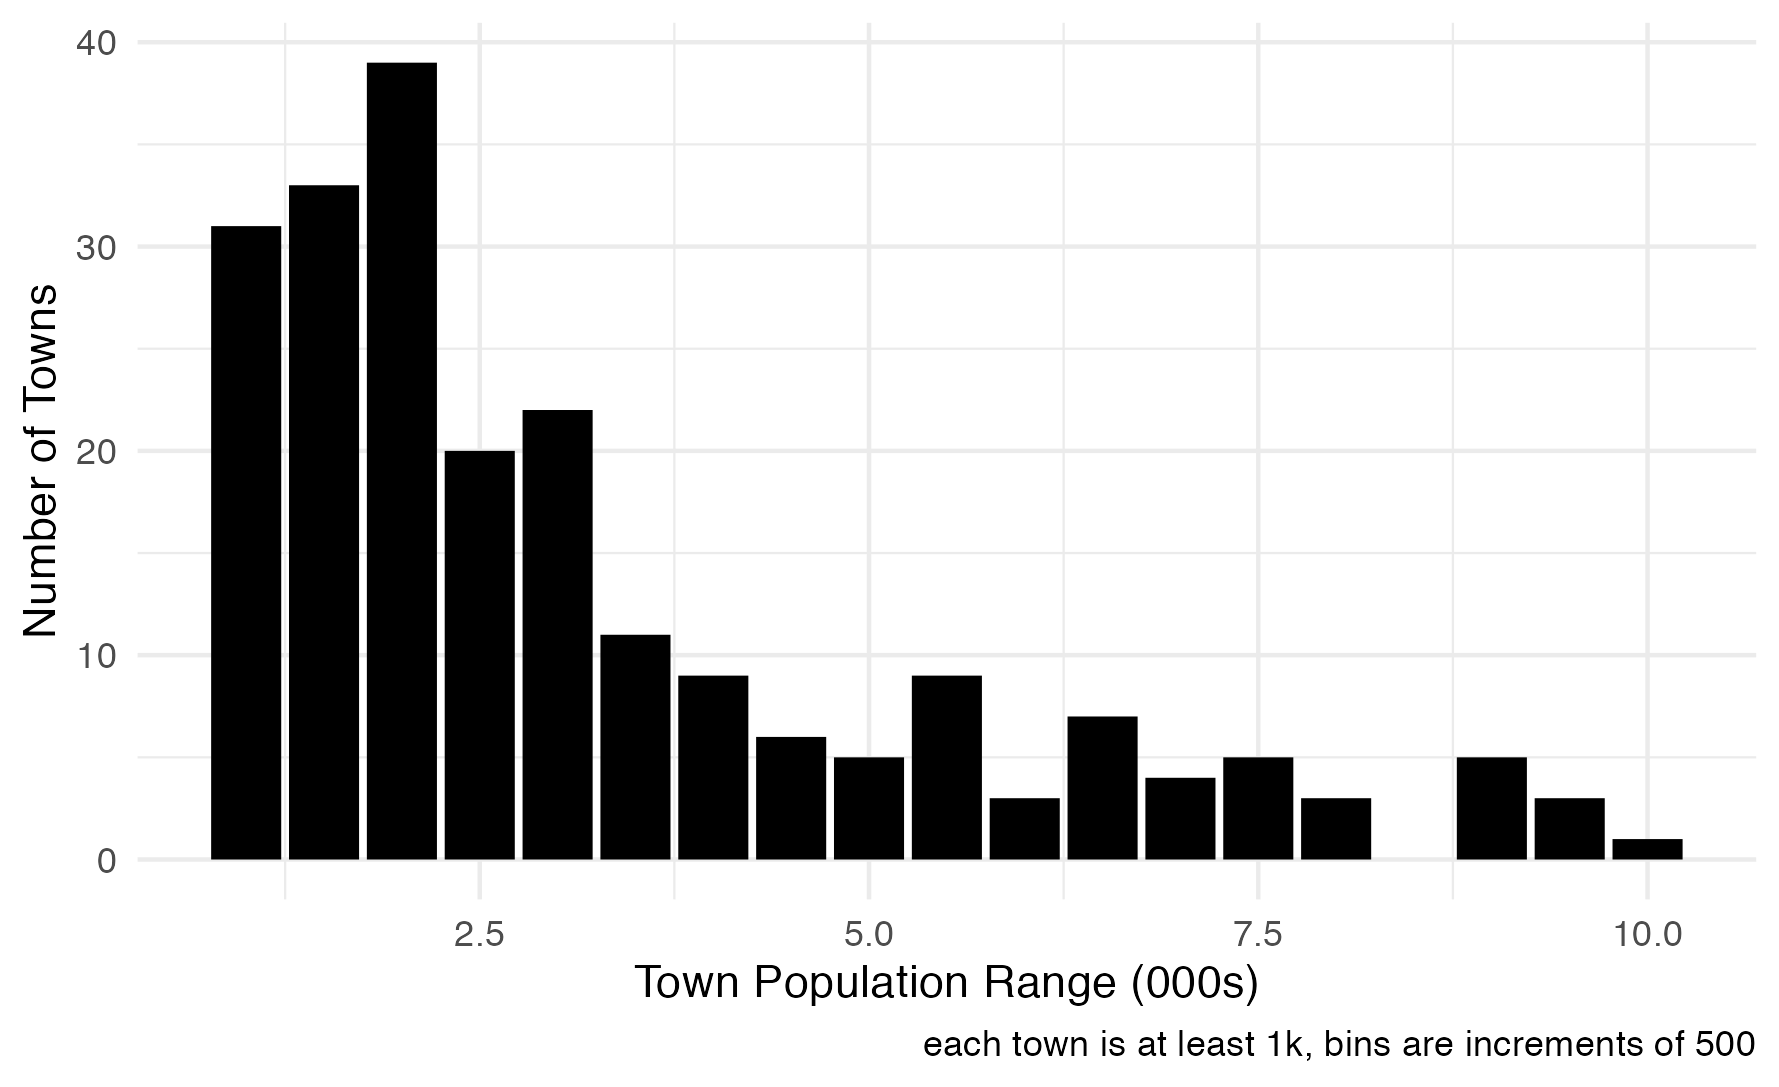
\includegraphics[width=0.85\linewidth]{figure2.png}
    \caption{Histogram of Town Populations}
    \label{figure1}
\end{figure}

\begin{figure}
    \centering
    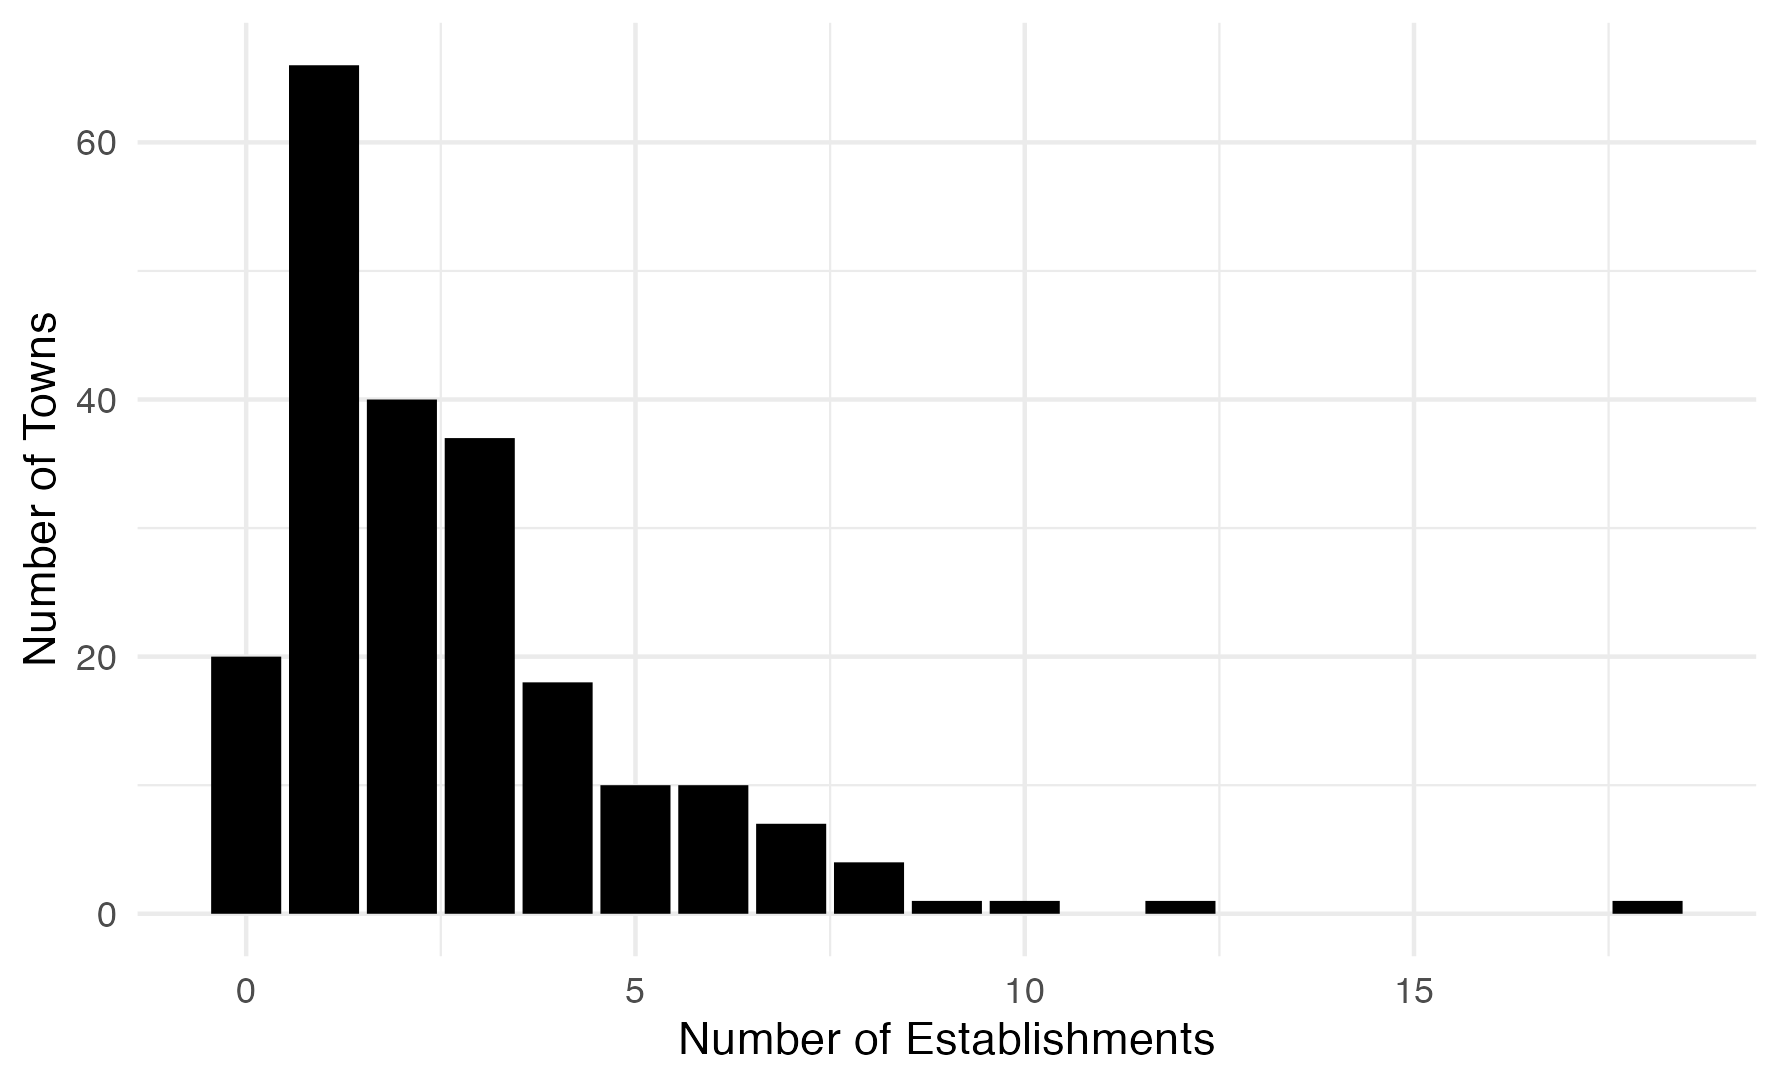
\includegraphics[width=0.85\linewidth]{table2Figure.png}
    \caption{Histogram of Dental Clinic Counts}
    \label{figure2}
\end{figure}

Table \ref{table1} displays descriptive statistics for market and demographic characteristics of towns in our sample. We can see that there is quite a bit of heterogeneity among towns in some of these characteristics. For example, the standard deviations and ranges of population percentage change, dwellings per kilometre, and average total income in 2020 suggest considerable differences in these characteristics across towns in the sample.

As in \citet{BresReiss}, we split these characteristics into those that determine market size and those that shift demand and cost. For market size determinants, we use total population, number of dwelling owners, population percentage change, and the percentage of individuals who commute outside the market for work. For demand shifters, we include all the demographic characteristics. For cost and demand shifters, we include the number of dwellings per kilometre, the median value of dwellings, and the regional dummies. The idea of the former two shifters is to get at the cost of renting space for dental clinics. For example, many dwellings per kilometre may indicate that space is scarce, driving up rental prices. Notably, both of these variables are related to living spaces, so we must assume that the values/prices of living spaces are correlated to the value/prices of commercial spaces. Furthermore, we include regional dummies in the demand and cost shifters to get at regional variation in both demand and the costs that dental clinics face. For example, there could be regional differences in labour markets that affect the wages dentists must pay to dental assistants and dental hygienists. Inclusion of regional dummies is also consistent with the provincial and territorial fee guides that are based on costs that dentists in respective provinces/territories face.

\begin{table}[ht]
\centering
\caption{Descriptive statistics for market and demographic characteristics}
\label{table1}
\begin{tabular}{@{}lllllll@{}}
\toprule
Variable & Mean & Std. dev. & Min & Max & Frequency \\ \midrule
\textit{Market characteristics} & & & & & \\
\# Dental clinics & 2.63 & 2.37 & 0 & 18 &  \\
Total population & 3.19 & 2.20 & 1.01 & 9.97 & \\
Dwelling owners (1000s) & 0.93 & 0.62 & 0.035 & 3.09 & \\
Population \% change (2016 to 2021) & 0.006 &	7.81 & -22.5 & 30.9 & \\
\% Commute outside market & 0.25 & 0.16 & 0.02 & 0.76 & \\
Dwellings per km & 418.56 &	150.18 & 107.46 & 1037.29 & \\
Median value of dwellings (\$1000s) & 248.37 & 144.79 &	50 & 1290 & \\ 
\textit{Demographic characteristics} & & & & & \\
Senior (65+) population & 24.91 & 8.49 & 2.70 & 54.60 & \\
Average \# children in families with children & 1.79 & 0.20 & 1.30 & 3 & \\
Average total income in 2020 (\$1000s) & 48.66 & 8.06 & 33.32 & 98.3 & \\
\% Has at least high school diploma & 0.77 & 0.083 & 0.37 &	0.96 & \\
Unemployed population (1000s) & 0.15 & 0.14 & 0 & 1.31 & \\
\textit{Regional dummies} & & & & & \\
Atlantic & & & & & 31 \\
Quebec & & & & & 35 \\
Ontario & & & & & 34 \\
Prairies & & & & & 94 \\
British Columbia & & & & & 22 \\ \bottomrule
\end{tabular}
\end{table}

\section{Model and Results}


\begin{table}[h]  
\begin{threeparttable}
\caption{Market and Businesses Counts} % title name of the table  
\centering % centering table  
\begin{tabular}{l c c } % creating 10 columns  
\hline\hline   
 Geography & Population Centres & Veterinarian Businesses   
\\ [0.5ex]  
\hline   
% Entering 1st row  
Canadian Provinces & 1014 & 1929 \\
Within CSA or surrounding 20km & 737 & 1573 \\
Within 10km of other Population Centre & 42 & 16 \\
Remaining Population Centres & 235 & 114 \\

Remaining PCs and surrounding 1km* & 235 & 186 \\

Remaining PCs and surrounding 2km  & 235 & 200 \\

Remaining PCs and surrounding 5km  & 235 & 209 \\

% [1ex] adds vertical space  
\hline % inserts single-line  
\end{tabular}  
\begin{tablenotes}
    \small  *This set of population centres including 186 veterinarian businesses was chosen for analysis. 
\end{tablenotes}
\end{threeparttable}
\end{table}  
%%%%%%%%%%%%%%%%%%%% Shuning's part starts here %%%%%%%%%%%%%%%%%%%%%%%%%%%%%%%%
\alert{*May need adjust the table number}
\section{Baseline estimates}

Table \ref{table4} reports ordered probit results. We include 36 parameters in the specification: three $\lambda$'s, eleven $\beta$'s, eight $\alpha$'s, six $\gamma_L$'s and eight $\gamma$'s. There are too many parameters in the specification. We intentionally introduce excess variables to incorporate alternative models of entrants' profits. And as a result, most coefficients are statistically insignificant. Bresnahan and Reiss (1991) claims that the insignificance of the coefficients is the evidence of homogeneous sample. 

Following Bresnahan and Reiss (1991), we first attempted to impose profit restriction that later entrants do not have higher profits (i.e., $\Bar{\Pi}_N\ge \Bar{\Pi}_{N+1}$). This constraint is equivalent to holding non-negative $\alpha$'s and $\gamma$'s, which is consistent with most of our estimates. However, when we continued to estimate the thresholds, the profit constraint gave us negative results. Therefore, the estimates in the following are without the constraint. 


\begin{table}[]
\setlength{\belowcaptionskip}{0.2cm}
\caption{Baseline ordered probit results}
\label{table4}
\resizebox{1.0\linewidth}{!}{
\begin{tabular}{@{}llll@{}}
\toprule
regTerm        & term                                                                          & value        & se          \\ \midrule
$\lambda1  $      & Owner                                                       & 0.043973899  & NaN         \\
$\lambda2 $       & Population.percentage.change..2016.to.2021                  & -0.436143255 & NaN         \\
$\lambda3 $       & Commuteout                                                  & 0.027521438  & NaN         \\
$\beta1 $         & Dwellingperkm                                               & -0.062095061 & 0.071309388 \\
$\beta2$          & Median.value.of.dwellings                              & 0.037305447  & 0.0609831   \\
\beta3 $         & AT                                                                            & 0.097142405  & 0.079628668 \\
$\beta4  $        & QC                                                                            & 0.031552684  & 0.079132411 \\
$\beta5 $         & ON                                                                            & -0.042358815 & 0.063016032 \\
$\beta6$          & BC                                                                            & -0.046860441 & 0.074170611 \\
$\beta7$          & TOTAL\_65.years.and.over                                           & -0.151082561 & 0.076904853 \\
$\beta8  $        & Average.number.of.children & 0.071261294  & 0.074405462 \\
$\beta9$          & Average.total.income.in.2020         & -0.034863728 & 0.064358258 \\
$\beta10  $       & Edatleasths                                                 & -0.004034581 & 0.081785671 \\
$\beta11 $        & Unemployed                                                  & 0.015146779  & 0.050779298 \\
$\gamma\_L1$      & Dwellingperkm                                               & 0.029801061  & 0.088273734 \\
$\gamma\_L2$      & Median.value.of.dwellings                              & -0.078494951 & 0.108233208 \\
$\gamma\_L3$      & AT                                                                            & -0.047652243 & 0.095537816 \\
$\gamma\_L4$      & QC                                                                            & -0.056257359 & 0.096401748 \\
$\gamma\_L5$      & ON                                                                            & -0.085085482 & 0.090216342 \\
$\gamma\_L6$      & BC                                                                            & 0.059009851  & 0.113684169 \\
$\alpha1 $        & V\_1 (a\_1)                                                                   & 0.022461159  & 0.061666657 \\
$\alpha2$         & F\_1 (g\_1)                                                                   & 0.056783217  & 0.024471124 \\
$\alpha3$         & V\_1 - V\_2 (a\_2)                                                            & -0.096496229 & 0.012076074 \\
$\alpha4$         & V\_2 - V\_3 (a\_3)                                                            & -0.017010608 & 0.012761205 \\
$\alpha5$         & V\_3 - V\_4 (a\_4)                                                            & -5.30E-04    & 0.018812347 \\
$\alpha6$         & V\_4 - V\_5 (a\_5)                                                            & -0.177999155 & 0.038348365 \\
$\alpha7  $       & V\_5 - V\_6 (a\_6)                                                            & 0.402106217  & 0.136979519 \\
$\alpha8$         & V\_6 - V\_7 (a\_7)                                                            & 0.024136647  & 0.002933992 \\
$\gamma\_n1$      & V\_7 - V\_8 (a\_8)                                                            & 0.037509481  & 0.096055429 \\
$\gamma\_n2$      & F\_2 - F\_1 (g\_2)                                                            & 0.346004586  & 0.043221486 \\
$\gamma\_n3$      & F\_3 - F\_2 (g\_3)                                                            & 0.096478143  & 0.015874658 \\
$\gamma\_n4$      & F\_4 - F\_3 (g\_4)                                                            & 0.17300883   & 0.028702114 \\
$\gamma\_n5$      & F\_5 - F\_4 (g\_5)                                                            & 0.128753531  & 0.032922849 \\
$\gamma\_n6$      & F\_6 - F\_5 (g\_6)                                                            & 0.078056261  & 0.031017745 \\
$\gamma\_n7$      & F\_7 - F\_6 (g\_7)                                                            & 0.034134112  & 0.031208544 \\
$\gamma\_n8$      & F\_8 - F\_7 (g\_8)                                                            & -0.007261887 & NaN         \\
Log likelihood & Log likelihood                                                                & 693.3082817  & NA          \\ \bottomrule
\end{tabular}}
\end{table}

Table \ref{table5} reports entry threshold estimates for specifications in table \ref{table4}. The formula to calculate the entry thresholds is given by
\begin{align}
    S_N=\frac{\hat{F_N}}{\hat{V_N}},
\end{align}

where a circumflex denotes the prediction from maximum likelihood estimates in table \ref{table4}. The optimal conduct in the market is given by the break-even condition. Unfortunately, our results are not satisfying as $S_N$ declines as $N$ increases, leading to an award situation that more entrants, more profit for each firm. Therefore, we cannot estimate the optimal number of dentists as $S_8$ is still less than 1. 

\begin{table}[ht]
\centering
\setlength{\belowcaptionskip}{0.2cm}
\caption{Entry threshold estimates}
\label{table5}
%\resizebox{1.0\linewidth}{!}{
\begin{tabular}{@{}lllll@{}}
\toprule
S\_N &             &  & S ratio    &             \\ \midrule
S\_1 & 0.353840027 &  & S\_1/S\_NA & NA          \\
S\_2 & 0.335408483 &  & S\_2/S\_1  & 0.947909952 \\
S\_3 & 0.332164911 &  & S\_3/S\_2  & 0.990329488 \\
S\_4 & 0.323690636 &  & S\_4/S\_3  & 0.974487747 \\
S\_5 & 0.317179656 &  & S\_5/S\_4  & 0.979885176 \\
S\_6 & 0.316076027 &  & S\_6/S\_5  & 0.996520492 \\
S\_7 & 0.308003448 &  & S\_7/S\_6  & 0.974460009 \\
S\_8 & 0.307994832 &  & S\_8/S\_7  & 0.999972028 \\ \bottomrule
\end{tabular}
\end{table}

Figure \ref{figure4} also shows the reverse results. It plots the ratio of the market size required to support 8 versus $N$ firms. For $N<8$, it varies from 0 to 1, depending on the estimated costs and variable profits. And the ratio increases to 1 as the number of firms approaches to 8. The reason why we have the reverse results dates back to estimates in table \ref{table4}, and the entry threshold ration increases in the ration of margins, entry costs, inefficiencies, and the slope.

\begin{figure}[ht]
    \centering
    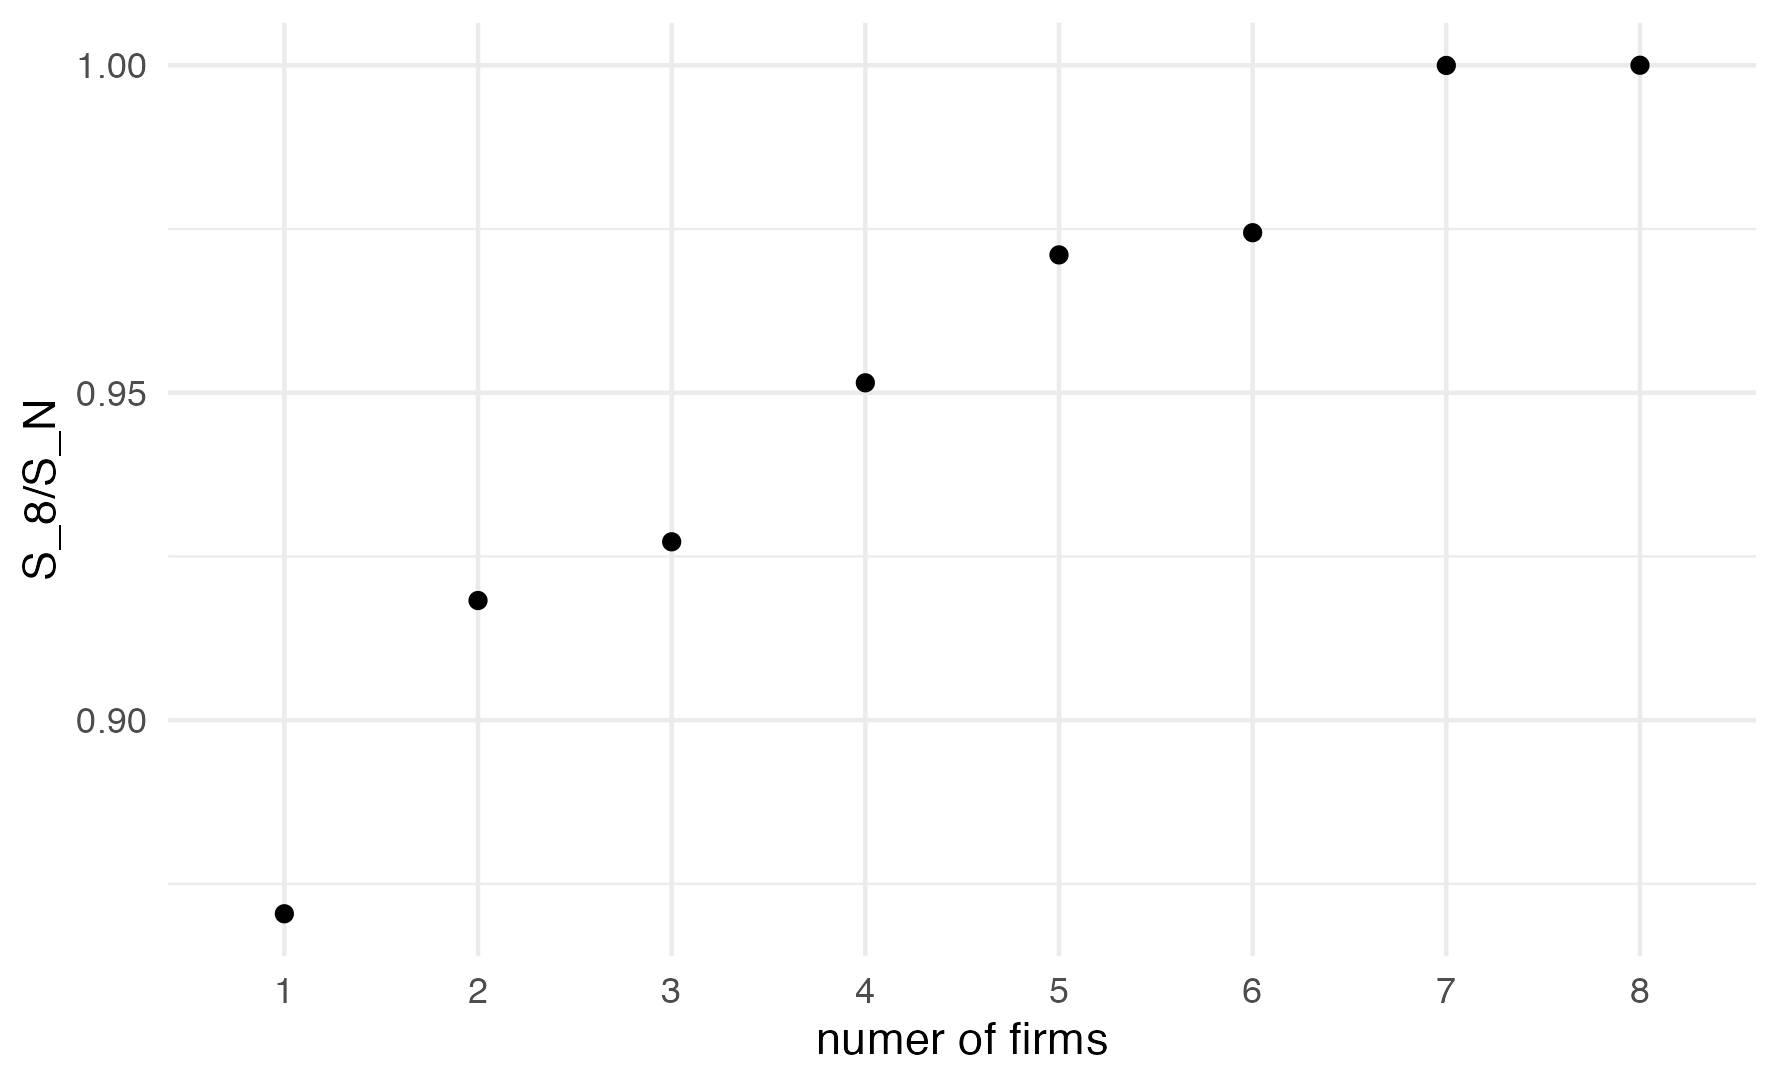
\includegraphics[width=.85 \textwidth]{IO/figure4.png}
    \caption{Industry ratios of $s_8$ to $s_N$ by $N$}
    \label{figure4}
\end{figure}

%(\textbf{I don't understand table 5b so i didn't write it.})

\section{Specification issues}
Table \ref{table4} and figure \ref{figure4} suggest that the eighth entrant does not change competitive conduct. So we test several profit shifters: entrants' fixed costs, town population, and local economic conditions. For each type of the profit shifters, we test if it can explain the difference in profits and therefore alter the entry threshold under maintained hypothesis.

Table \ref{table678} summarizes all the test results. We first test the null that same fixed costs for every firm. As the likelihood ratio test statistic (LRT) is way above the threshold, we should reject the null hypothesis of equal fixed costs, this is consistent with significant $\gamma$'s in table \ref{table4}. Moreover, the constrained entry threshold ratios are slightly bigger than unconstrained estimates due to the constrained fixed costs.

Second, we test the effect of market size $S(Y)$ described by town population. The null hypothesis is that the coefficients of market size are all 0 and it is easily rejected by the test statistic. After removing all the market size effects, the ratios of entry threshold increase slightly just as in the first exercise.

Third, we test for the effects of local economic conditions. While we reject the null that eliminating the effects of local economic conditions, the variation in the constrained ratios of entry thresholds is much bigger, ranging from 0.38 to 1.31. This result reflects the significant contribution of overall local economic conditions in variable profits. 

\begin{table}[htbp]
\centering
\caption{Likelihood ratio tests for different hypotheses}
\label{table678}
\resizebox{1.0\linewidth}{!}{
\begin{tabular}{cccc}
\toprule
Name                      & Same fixed costs & Market size exclusion                           & Local economic condition exclusion  \\ \midrule
LikelihoodValue           & 825.3121082 & 904.7645924                                     & 904.7645924                                                                                                                                                                     \\
LRT                       & 264.0076529 & 422.9126214                                     & 422.9126214                                                                                                                                                                     \\
DegreesFreedom/OmittedVar & 7           & \makecell{Owner, Population.\\percentage.change, Commuteout} & \makecell{Dwellingperkm, Median.value.of.dwellings,\\ AT, QC, ON, BC, 65.years.and.over, \\Average.number.of.children, \\Average.total.income, Edatleasths, Unemployed} \\
S\_2/S\_1                 & 0.993097185 & 0.995404937                                     & 0.376140367                                                                                                                                                                     \\
S\_3/S\_2                 & 0.992671884 & 0.996766619                                     & 0.805254603                                                                                                                                                                     \\
S\_4/S\_3                 & 0.995720775 & 0.997388563                                     & 0.804219601                                                                                                                                                                     \\
S\_5/S\_4                 & 0.997879475 & 0.998288174                                     & 1.208973714                                                                                                                                                                     \\
S\_6/S\_5                 & 1.00204492  & 1.000528132                                     & 1.089678467                                                                                                                                                                     \\
S\_7/S\_6                 & 1.001986975 & 1.000064656                                     & 1.185406988                                                                                                                                                                     \\
S\_8/S\_7                 & 1.002495309 & 1.004060511                                     & 1.311457457  \\ \bottomrule                                                                    
\end{tabular}}
\end{table}

Finally, we test the market criteria. If the markets are too close to each other, then the migration of consumers may bias our estimates. The number of population commuting out proxies the migration, but it presents an insignificant weak positive correlation with the market size in table \ref{table4} (weird). Besides, the nearby supply-side sources could also affect the demand-side analysis. Hence, we explore two other market criteria, one weaker (2km away) and one stronger (5km away). Table \ref{table9} reports the results under alternative market definitions. As is shown in table \ref{table9}, none of the specification exhibits significant difference in ratios of thresholds for more than 2 firms from our baseline estimates (table \ref{table5}).  However, the second entrant has relatively lower margin than before as we observe higher $S_2/S_1$ in table \ref{table9} if we change the market criterion. Overall, the results from table \ref{table9} supports our previous market specification. 

\begin{table}[ht]
\centering
\caption{Entry thresholds for alternative market definitions}
\label{table9}
\begin{tabular}{@{}lll@{}}
\toprule
Distance & 2km         & 5km         \\ \midrule
S\_2/S\_1    & 1.004616399 & 0.993312244 \\
S\_3/S\_2    & 1.001384557 & 0.995949242 \\
S\_4/S\_3    & 1.005929137 & 0.99682532  \\
S\_5/S\_4    & 1.0031106   & 0.993926681 \\
S\_6/S\_5    & 1.00523086  & 0.996596202 \\
S\_7/S\_6    & 0.993084012 & 0.993310898 \\
S\_8/S\_7    & 1.000234026 & 1.010782519 \\ \bottomrule
\end{tabular}
\end{table}
%%%%%%%%%%%%%%%%%%%%%%

\section{Conclusion}
In this paper, we apply the analysis of market concentration and competition of Bresnahan and Reiss (1991) to the Canadian dental industry. Using data on isolated Canadian markets, we employ an ordered probit model to estimate the number of dental clinics in each market and use the results to compute entry thresholds for new entrants under different market structures. However, we do not obtain very precise results for variable profits and fixed costs from the ordered probit model and we find that entry thresholds decrease as markets become more concentrated. As such, we are unfortunately unable to make very sound conclusions about market concentration and competition in the Canadian dental industry.

\newpage
\printbibliography

\newpage
\section*{Appendix}
\subsection*{Data Collection Process}




\end{document}
